\documentclass[crop,tikz]{standalone}

\usepackage{fontspec}
\setmainfont{texgyrepagella}[
  Extension = .otf,
  UprightFont = *-regular,
  BoldFont = *-bold,
  ItalicFont = *-italic,
  BoldItalicFont = *-bolditalic,
]

\usepackage{tikz}
\usetikzlibrary{decorations.pathreplacing,calligraphy}
\usetikzlibrary{calc}

\makeatletter % https://tex.stackexchange.com/a/38995/121799
\tikzset{
  use path/.code={\pgfsyssoftpath@setcurrentpath{#1}}
}
\makeatother
\tikzset{reverseclip/.style={insert path={(current bounding box.north
        east) rectangle (current bounding box.south west)}}}

\pgfdeclarelayer{bg}
\pgfsetlayers{bg,main}


\begin{document}
    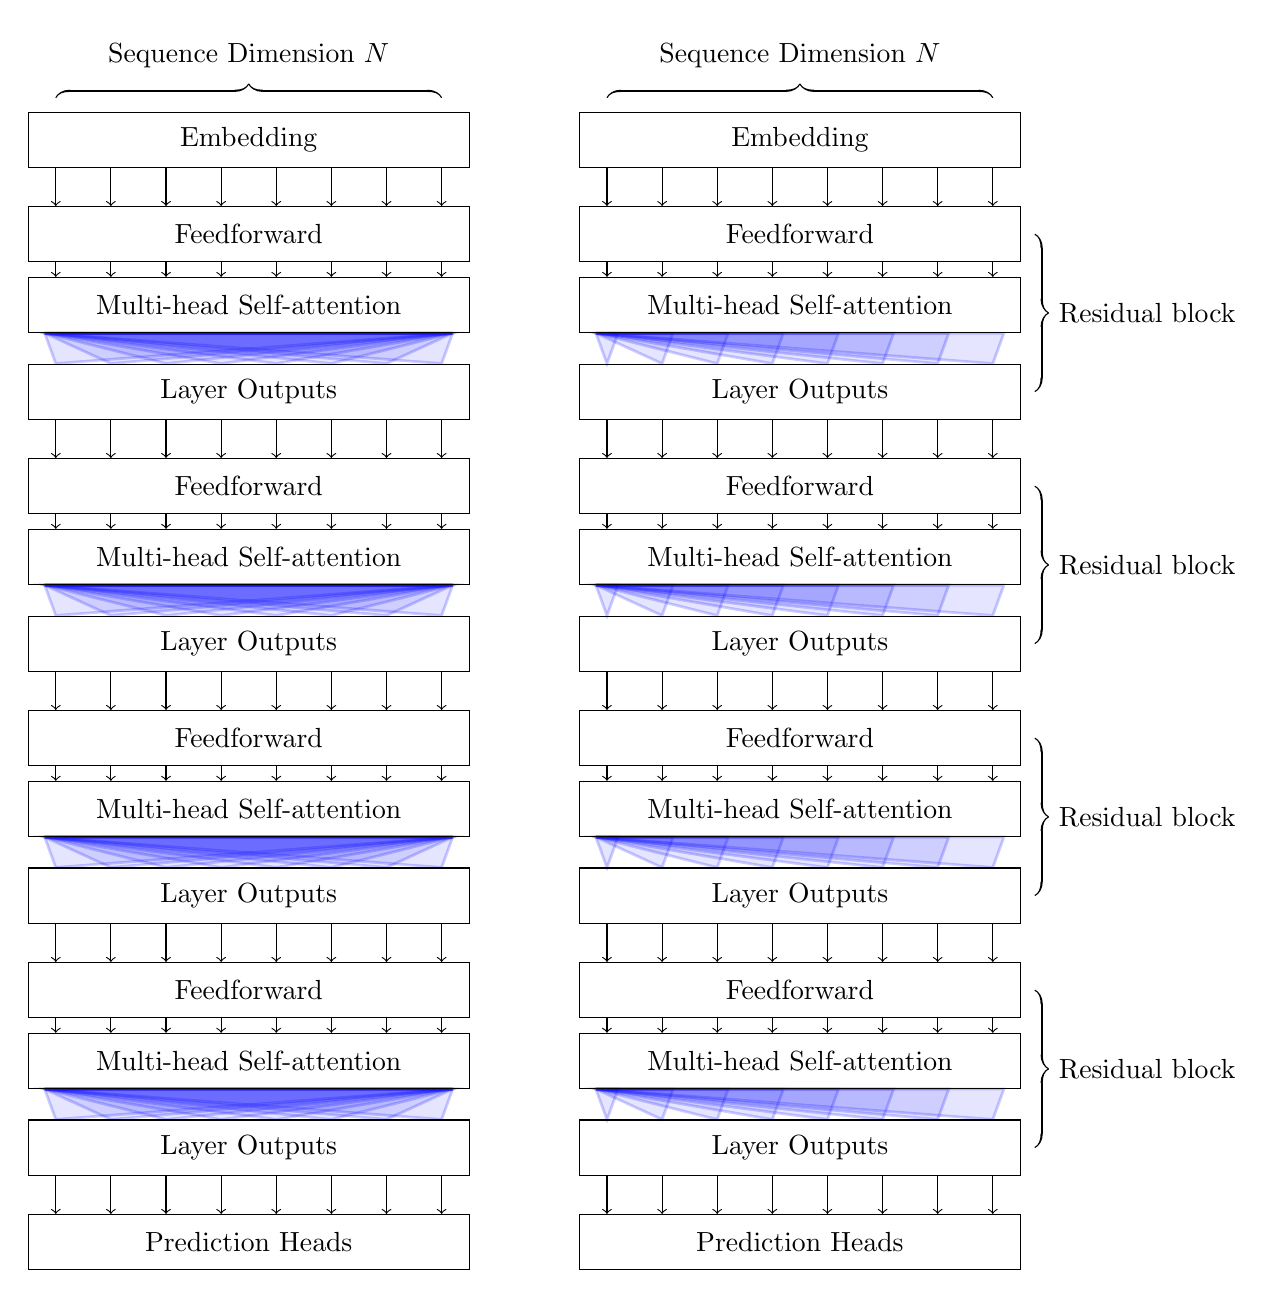
\begin{tikzpicture}
        \tikzstyle{every node}=[minimum width=0.7cm, minimum height=0.7cm,anchor=west]

        \begin{scope}[shift={(-3cm,0)}]

            \node[draw,minimum width=5.6cm] at (0, 1.2cm) {Embedding};
            \foreach \x in {0,...,7} {
                \node (o_0_\x) at (\x*0.7 cm, 1.2cm) {};
            }
            \foreach \lay / \layy in {0/1,1/2,2/3,3/4} {
                \begin{scope}[shift={(0, \lay*-3.2cm)}]
                    \node[draw,minimum width=5.6cm] at (0,0) {Feedforward};
                    \node[draw,minimum width=5.6cm] at (0,-0.9cm) {Multi-head Self-attention};
                    \node[draw,minimum width=5.6cm] at (0,-2cm){Layer Outputs};
                    \foreach \x in {0,...,7} {
                        \begin{scope}[shift={(\x*0.7 cm, 0)}]
                            \node (ff_\layy_\x) at (0, 0) {};
                            \node (a1_\layy_\x) at (0, -0.9cm) {};
                            \node (o_\layy_\x) at (0, -2cm) {};
                        \end{scope}
                    }
                \end{scope}
            }

            \begin{scope}[shift={(0, 4*-3.2cm)}]
                \node[draw,minimum width=5.6cm] at (0, 0) {Prediction Heads};
                \foreach \x in {0,...,7} {
                    \node (p_0_\x) at (\x*0.7 cm, 0) {};
                }
            \end{scope}

            \foreach \lay / \layy in {0/1,1/2,2/3,3/4} {
                \foreach \x in {0,...,7} {
                    \draw[->] (o_\lay_\x.south) -- (ff_\layy_\x.north);
                    \draw[->] (ff_\layy_\x.south) -- (a1_\layy_\x.north);
                    \begin{pgfonlayer}{bg}
                        \begin{scope}[every path/.append style={draw=blue,fill=blue,fill opacity=0.1,draw opacity=0.2}, blend group=darken]
                            \fill[blue] (o_\layy_\x.north) -- ([xshift=-4pt]a1_\layy_0.south) -- ([xshift=4pt]a1_\layy_7.south) -- cycle;
                        \end{scope}
                    \end{pgfonlayer}
                }
            }
            \foreach \x in {0,...,7} {
                \draw[->] (o_4_\x.south) -- (p_0_\x.north);
            }

            \draw[thick,decorate,decoration={calligraphic brace,raise=5pt, amplitude=5pt}] (o_0_0.north) -- node[draw=none,above=10pt] {Sequence Dimension $N$} (o_0_7.north) {};


        \end{scope}

        \begin{scope}[shift={(4cm,0)}]

            \node[draw,minimum width=5.6cm] at (0, 1.2cm) {Embedding};
            \foreach \x in {0,...,7} {
                \node (o_0_\x) at (\x*0.7 cm, 1.2cm) {};
            }
            \foreach \lay / \layy in {0/1,1/2,2/3,3/4} {
                \begin{scope}[shift={(0, \lay*-3.2cm)}]
                    \node[draw,minimum width=5.6cm] at (0,0) {Feedforward};
                    \node[draw,minimum width=5.6cm] at (0,-0.9cm) {Multi-head Self-attention};
                    \node[draw,minimum width=5.6cm] at (0,-2cm){Layer Outputs};
                    \foreach \x in {0,...,7} {
                        \begin{scope}[shift={(\x*0.7 cm, 0)}]
                            \node (ff_\layy_\x) at (0, 0) {};
                            \node (a1_\layy_\x) at (0, -0.9cm) {};
                            \node (o_\layy_\x) at (0, -2cm) {};
                        \end{scope}
                    }
                \end{scope}
            }

            \begin{scope}[shift={(0, 4*-3.2cm)}]
                \node[draw,minimum width=5.6cm] at (0, 0) {Prediction Heads};
                \foreach \x in {0,...,7} {
                    \node (p_0_\x) at (\x*0.7 cm, 0) {};
                }
            \end{scope}

            \foreach \lay / \layy in {0/1,1/2,2/3,3/4} {
                \draw[thick,decorate,decoration={calligraphic brace,raise=5pt, amplitude=5pt}] (ff_\layy_7.east) -- node[draw=none,anchor=west,right=10pt] {Residual block} (o_\layy_7.east);
                \foreach \x in {0,...,7} {
                    \draw[->] (o_\lay_\x.south) -- (ff_\layy_\x.north);
                    \draw[->] (ff_\layy_\x.south) -- (a1_\layy_\x.north);
                    \begin{pgfonlayer}{bg}
                        \begin{scope}[every path/.append style={draw=blue,fill=blue,fill opacity=0.1,draw opacity=0.2}, blend group=darken]
                            \fill[blue] (o_\layy_\x.north) -- ([xshift=-4pt]a1_\layy_0.south) -- ([xshift=4pt]a1_\layy_\x.south) -- cycle;
                        \end{scope}
                    \end{pgfonlayer}
                }
            }
            \foreach \x in {0,...,7} {
                \draw[->] (o_4_\x.south) -- (p_0_\x.north);
            }

            \draw[thick,decorate,decoration={calligraphic brace,raise=5pt, amplitude=5pt}] (o_0_0.north) -- node[draw=none,above=10pt] {Sequence Dimension $N$} (o_0_7.north);
        \end{scope}

    \end{tikzpicture}
\end{document}
